In the curriculum of the Mechanical Engineering degree program at the Department of Engineering and Technological Research (DIIT) of UNLaM, this subject is the link between the first ones specific to the specialty with the basic ones in which tools of algebra, mathematical analysis, numerical calculus, and Newtonian mechanics are taught. The scheme of immediate correlations to the General Mechanics subject, which shows Figure \ref{fig:correlativas}, makes it clear that this subject must have among its objectives to show the student how these tools have an application in their area of interest.

\begin{figure}[!ht]
\centering
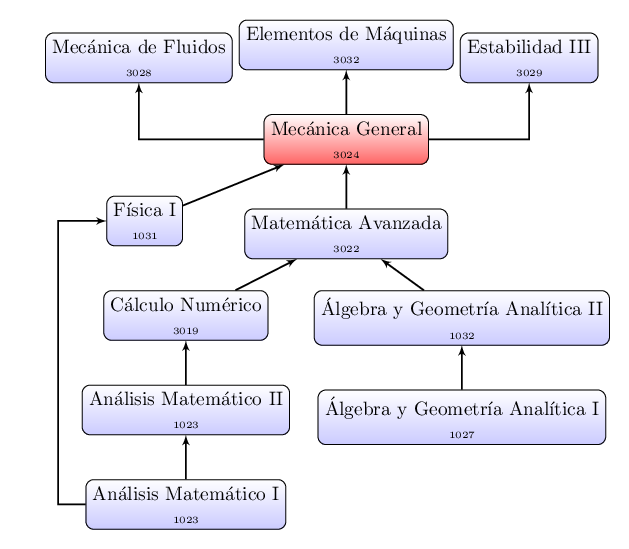
\includegraphics[width=3in]{figuras/correlativas.png}
\caption{Preceded by subjects of algebra, analysis, and physics, General Mechanics is the first in which such knowledge is applied to mechanical engineering.}
\label{fig:correlativas}
\end{figure}

The subject trains students in the ability to model the physics of simple mechanical systems. Modeling is understood as a series of procedures with which a simplified scheme of physics is constructed based on a semi-quantitative evaluation of the forces and fields that act on the system as well as the constraints that limit its degrees of freedom. With such information, some of these are prioritized and others are discarded to arrive at the aforementioned scheme. Having such a model allows:
\begin{itemize}
    \item to choose generalized coordinates to describe the relevant degrees of freedom,
    \item to write mathematical relationships between them that account for constraints,
    \item to describe generalized forces that are not the effect of fields (gravitational, electromagnetic, etc.),
    \item and to describe the potential and kinetic energy of the system as a whole.
\end{itemize}


After performing the above, the Euler-Lagrange formalism is demonstrated and put into practice in the course to obtain a set of differential equations that describe the dynamics of the system and/or the mechanical stresses that each of its components must withstand at each instant of time.

From what has been exposed in the preceding paragraphs, it is evident that the subject matter of the course object of this work is circumscribed to the conventional one of rational mechanics courses as detailed in its canonical reference literature \cite{landau}. It is not in the subject matter but in its didactic methodology where innovation was made.

\subsection{The blackboard, the only didactic tool}

Traditionally, the systems worked on in rational mechanics courses are relatively simple to limit the time and/or difficulty of mathematical analysis and/or algebra calculations required by the steps commented in the previous paragraph. But this extreme simplification leads to a noticeable jump in the complexity required to model mechanical devices, fluid dynamics, or rigid structures, the respective subjects of the courses subsequent to General Mechanics (see Figure \ref{fig:correlativas}).

The limitation to complexity is imposed by what the teacher can calculate on the blackboard during a class. As they are erased successively, they not only prevent the student from using a reference of something that is no longer in sight, but also impose on them to devote a good part of their attention to not making mistakes when transcribing what is written there into their notebook. This paper support, in turn, limits the length and complexity of the problems that can be proposed to students to exercise what they have learned. What summarizes the preceding paragraph is nothing more than the procedure in the teaching of science or engineering courses at the university level that has been almost unchanged since the 19th century to the present day.


\subsection{Computer-based didactic tools}

The steps before and after obtaining a system of differential equations that describe the dynamics and stresses for a complex mechanical model can be performed with computer-based tools, but they are different for each case. To solve and analyze the result of the equations, the tools learned in the Numerical Calculus subject, previously taken before General Mechanics, and ubiquitous graphing tools to visualize the temporal evolution of different magnitudes are applied. Although it is true that numerical calculus is occasionally used in exercises \cite{mirasso-raichman, caligaris-rodriguez}, it is rarely used by the teacher during class. This is a missed opportunity to better exemplify and deepen the analysis of the behavior of the modeled systems.

But if the application of numerical calculus during classes is rare, the use of computer algebra systems (CAS) is even rarer. These systems allow automating all the mathematical procedures required for modeling: from defining degrees of freedom, coordinate systems, fields, and external forces to the model to building the system of differential equations for the dynamics. Using them to solve linear algebra and mathematical analysis calculations allows to remove the emphasis on these and focus the attention of the teacher and students on the subject matter of the course.

However, the daily reality of our classrooms is that these calculations continue to be done manually on the blackboard or on paper during classes, ignoring the use of computers. Insisting on this procedure at the university level would be analogous to depriving students of the use of pocket calculators to perform arithmetic procedures learned at the primary level. It is an anachronism in the third decade of the 21st century.

\subsection{Code recycling}

The above can be misinterpreted as a mere call to use computers as an analog of the pocket calculator, replacing the results of the calculations required to solve exercises on paper. This would be an underutilization of such a resource in the class, repeating the pattern followed by most computer users who ignore a fundamental aspect of computing in their daily use.

The digital computer was invented during World War II to perform numerical calculations that were manually defined in each execution, operating as a faster calculator with the ability to automate some of the numerical manipulation processes. But since the middle of the last century, it has acquired the ability to operate under a series of instructions stored in its memory on how to process both numerical and other information. Such instructions are called programs, and they are written in a code that respects the syntax of a certain language.

Modern high-level languages allow writing a single code incorporating all the procedures required for the resolution and analysis of a rational mechanics problem. This includes from the assumptions made to simplify the physics of the problem to the analysis with graphs of its dynamics and mechanical stresses, passing through all the intermediate algebraic and numerical calculations.

Starting from the objective that students exploit this tool, the course had as its methodology to avoid paper work and instead develop the ability to write in a single code the set of operations required to solve exercises. In class, the teacher explained synchronously examples of codes that perform all the procedures required to model a mechanical system. In each class, a guide to solvable exercises is provided by making small modifications to the code.














% En el plan de la carrera de grado en Ingeniería Mecánica del Departamento de Ingeniería e Investigaciones Tecnológicas (DIIT) de la UNLaM esta asignatura es el nexo entre las primeras propias de la especialidad con las básicas en las que se imparten herramientas de álgebra, análisis matemático, cálculo numérico, y mecánica Newtoniana. El esquema de correlatividades inmediatas a la asignatura Mecánica General, que muestra la figura \ref{fig:correlativas}, deja en claro que esta debe tener entre sus objetivos el mostrar al alumno cómo dichas herramientas tienen aplicación en su tema de interés.

% \begin{figure}[!ht]
% \centering
% 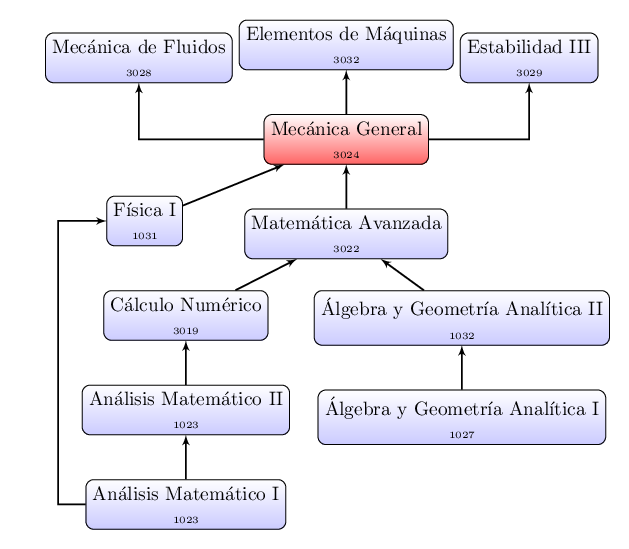
\includegraphics[width=3in]{figuras/correlativas.png}
% \caption{Precedida de asignaturas de álgebra, análisis y física, Mecánica General es la primera en que se aplican tales conocimientos a la ingeniería mecánica.}
% \label{fig:correlativas}
% \end{figure}

% La asignatura entrena a los alumnos en la habilidad de modelizar la física de sistemas mecánicos simples. Se entiende por modelizar el realizar una serie de procedimientos con los que se construye un esquema simplificado de la física partiendo de una evaluación semi-cuantitativa de las fuerzas y campos que actúan sobre el sistema así como de las ligaduras que limitan sus grados de libertad. Con tal información se priorizan algunas de estas y se descartan otras para arribar al esquema mencionado. Disponer de tal modelo permite:
% \begin{itemize}
%     \item elegir coordenadas generalizadas para describir los grados de libertad relevantes,
%     \item escribir relaciones matemáticas entre estas que den cuenta de ligaduras,
%     \item describir las fuerzas generalizadas que no sean efecto de campos (gravitatorio, electromagnéticos, etc.),
%     \item y describir la energía potencial y cinética del sistema en su conjunto.
% \end{itemize}

% Tras realizar lo anterior se demuestra y se pone en práctica en el curso el formalismo de Euler-Lagrange para obtener un conjunto de ecuaciones diferenciales que describen la dinámica del sistema y/o los esfuerzos mecánicos que cada uno de sus componentes debe soportar en cada instante de tiempo.

% De lo expuesto en los párrafos precedentes se evidencia que la temática del curso objeto de este trabajo está circunscrita a la convencional de los cursos de mecánica racional como se detalla en su literatura canónica de referencia \cite{landau}. No es en la temática sino en su metodología didáctica donde se hizo una innovación.

% \subsection{El pizarrón, única herramienta didáctica}

% Tradicionalmente los sistemas que se trabajan en los cursos de mecánica racional son relativamente simples para acotar el tiempo y/o dificultad de los cálculos de análisis matemático y/o de álgebra que requieren los pasos comentados en el párrafo anterior. Pero esta simplificación extrema lleva a un notorio salto en la complejidad de la que requiere modelar de dispositivos mecánicos, la dinámica de fluidos o a estructuras rígidas, las respectivas temáticas de las asignaturas subsiguientes a Mecánica General (ver figura \ref{fig:correlativas}).

% La limitación a la complejidad la impone lo que el docente puede, en la duración de una clase, calcular en el pizarrón. Estos al irse borrando sucesivamente no sólo impide al alumno servirse de referencia de algo que ya no está a la vista sino que además le impone dedicar buena parte de su atención a no cometer errores al transcribir lo allí escrito en su cuaderno. Este soporte en papel a su vez limita la extensión y complejidad de los problemas que pueden proponerse al alumnado para ejercitar lo aprendido. 
% Lo  que sintetiza el párrafo precedente no es otra cosa que el proceder en el dictado de clases de ciencias o ingeniería a nivel universitario que se reproduce casi en forma inalterada desde el siglo XIX hasta nuestros días.

% \subsection{Herramientas didácticas informáticas}

% Los pasos previos y posteriores al obtener un sistema de ecuaciones diferenciales que describen la dinámica y esfuerzos para un modelo mecánico complejo pueden realizarse con herramientas informáticas, pero que son distintas para cada caso.
% Para resolver y analizar el resultado de las ecuaciones se aplican las herramientas aprendidas en la asignatura Cálculo Numérico, cursada previamente a Mecánica General, y las ubicuas de graficación para visualizar la evolución temporal de distintas magnitudes. Si bien es cierto que el cálculo numérico se aprovecha ocasionalmente en la ejercitación \cite{mirasso-raichman, caligaris-rodriguez}, este rara vez es utilizado por el docente durante la clase. Se pierde así una oportunidad de ejemplificar mejor y profundizar el análisis del comportamiento de los sistemas modelados.

% Pero si es rara la aplicación del cálculo numérico durante las clases lo es aún más el uso de sistemas de álgebra computacional (Computer Algebra Systems o CAS, en inglés), que permiten automatizar todos los procedimientos matemáticos que requiere la modelización: desde definir grados de libertad, sistema de coordenadas, campos y fuerzas externas al modelo hasta construir el sistema de ecuaciones diferenciales para la dinámica. El utilizarlos para resolver cálculos de álgebra lineal y análisis matemático permite quitar el énfasis sobre estos y centrar la atención del docente y alumnos en la temática propia de la asignatura.

% Pero la realidad cotidiana de nuestras aulas es que durante las clases dichos cálculos se continúan realizando manualmente en el pizarrón o en papel obviando el uso de la informática. Empeñarse en ese proceder en el nivel universitario sería análogo al de privar al alumnado del uso de calculadoras de bolsillo para realizar procedimientos aritméticos aprendidos en el nivel primario. Todo un anacronismo en la tercera década del siglo XXI.

% \subsection{Reciclado del código}

% Lo precedente puede interpretarse erróneamente como un mero llamado a utilizar la informática como un análogo de la calculadora de bolsillo, supliendo resultados de los cálculos que demanda la resolución de ejercicios en papel. Eso sería una infrautilización de tal recurso en la clase, repitiendo el patrón que sigue la mayor parte de los usuarios de computadoras que obvian en su uso cotidiano un aspecto fundamental de la informática.

% La computadora digital se inventó en la Segunda Guerra Mundial con el fin de realizar cálculos numéricos que se definían manualmente en cada ejecución operando como una calculadora más rápida y con capacidad de automatizar algunos de los procesos de manipulación numérica.  Pero desde la mitad del siglo pasado adquirió la capacidad de operar bajo una serie de instrucciones almacenadas en su memoria sobre cómo procesar información tanto numérica como de otra índole. Tales instrucciones reciben el nombre de programa, y se escriben en un código que respeta la sintaxis de un determinado lenguaje.

% Los lenguajes modernos de alto nivel permiten escribir un único código incorporando  todos los procedimientos que requiere la resolución y el análisis de un problema de mecánica racional. Esto abarca desde las aproximaciones asumidas para simplificar la física del mismo hasta el análisis con gráficas de su dinámica y esfuerzos mecánicos pasando por todos los cálculos algebraicos y numéricos intermedios.

% Partiendo del objetivo de que los alumnos exploten esta herramienta el curso tuvo por metodología el obviar el trabajo en papel y en su lugar desarrollar la habilidad de escribir en un único código el conjunto de operaciones que requiere la resolución de ejercicios. En clase el docente explicó en forma sincrónica ejemplos de códigos que realizan todos los procedimientos requeridos para modelar un sistema mecánico. En cada clase se provee una guía de ejercicios resolubles haciendo pequeñas modificaciones al código provisto por el docente en esa fecha. Sucesivos ejercicios de complejidad creciente requieren pequeñas modificaciones respecto al código con que se resolvió el anterior. Esta reutilización del código permite un mejor aprovechamiento del tiempo y esfuerzo del alumno que en resoluciones en papel donde debe repetir procedimientos ya realizados en anteriores oportunidades. Clase a clase el alumnado construye una biblioteca de códigos con capacidades crecientes de análisis \cite{Barba2019}.

% Hay que aclarar que no se forma al alumno en programación para que cree aplicaciones o algoritmos, lo que se denomina programming en inglés. Lo que se busca es que puedan codificar  (por coding en inglés) las instrucciones para que la computadora realice tareas específicas, en particular cálculos para la ingeniería mecánica.

% Algunos alumnos archivan sus resoluciones de ejercicios resueltas en papel como referencia en caso de que se presente una problemática similar más adelante en el cursado de la carrera o en la vida profesional. En los hechos esto rara vez sucede y si recurren en el futuro a algún material relacionado a la asignatura es a su bibliografía, que por lo expuesto anteriormente carece de ejemplos adaptables a modelos más complejos que los comúnmente tratados en la asignatura. Por contrapartida un código es fácilmente aplicable al análisis de una problemática profesional análoga a las vistas en el curso. Al figurar en forma explícita las instrucciones para realizar cada paso del procedimiento es sencillo de revisar, expandir y modificar.